\chapter{Fabrication of Depletion-Mode HEMT Devices}

\section{Overview of the Fabrication Workflow}

The depletion--mode HEMTs characterised in this report were fabricated
using the standard III--V device process established within the Leeds
Nanotechnology Cleanroom. The workflow follows the routine sequence used
for GaAs/AlGaAs transistors in this facility, comprising mesa definition,
ohmic contact formation, contact annealing and Schottky--gate
metallisation. This well-established procedure was followed without
modification and carried out over four laboratory sessions. The devices
produced through this workflow provide a reliable baseline against which
the behaviour of devices with different structures and dimensions can be compared.

\vspace{3mm}

% FIGURE: Cleanroom process overview (optional)


\section{Mesa Definition and Isolation Etch}

The fabrication process began with the electrical isolation of individual device
regions through mesa etching. Prior to lithography, the GaAs wafer was
cleaned sequentially in acetone, isopropanol and deionised water to
remove organic residues and ensure good resist adhesion. A positive
 photoresist was then spun onto the sample at 3000rpm, soft-baked at
 approximately 115\,$^{\circ}$C and patterned using MLA exposure (Figure~\ref{fig:mesa_mask}).

\vspace{2mm}
\begin{figure}[htbp]
  \centering
  \includegraphics[width=0.5\linewidth]{figures/fabrication_images/mesa_mask.jpg}
  \caption{Mesa lithography mask used for defining isolated device regions. (Post-Development)}
  \label{fig:mesa_mask}
\end{figure}

Following development, the mesa pattern was transferred into the wafer
using a sulphuric acid, hydrogen peroxide and water wet-etch solution.
This mixture provides an isotropic etch suitable for the shallow
$\approx 200\,$nm recess required to isolate the active GaAs/AlGaAs
region from the surrounding substrate. The etched depth was measured as
178\,nm using the Alpha-Step profilometer, close to the intended value.
After etching, the remaining photoresist was stripped to leave sharply
defined mesas ready for ohmic contact formation.

\vspace{3mm}



\section{Ohmic Contact Formation}

Low-resistance ohmic contacts were formed using a dual-layer resist stack
consisting of LOR and S1803. This combination creates a controlled
undercut profile that ensures clean metal lift-off. The source and drain
regions were patterned by photolithography and developed to reveal the
contact openings.
% Dual-layer resist stack showing undercut for clean lift-off
\begin{figure}[htbp]
  \centering
  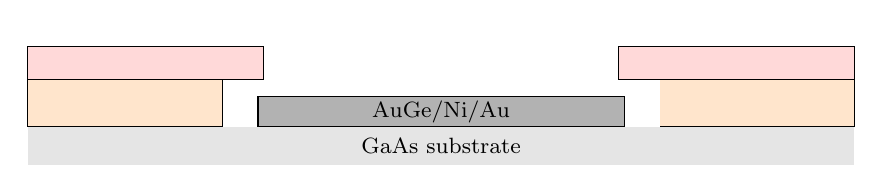
\begin{tikzpicture}[x=1.5cm,y=0.6cm,font=\footnotesize]
    % Dimensions
    \def\w{7}
    \def\hsub{0.8}
    \def\hlor{1.0}
    \def\hs1803{0.7}
    \def\gap{0.35}
    \def\xL{2.0}
    \def\xR{5.0}

    % Keep bounding box tight to the main drawing so labels don't shift centering
    \path[use as bounding box] (0,0) rectangle (\w,\hsub+\hlor+\hs1803+0.4);

    % Substrate (GaAs)
    \fill[gray!20] (0,0) rectangle (\w,\hsub);
    \node at (3.5,0.4) {GaAs substrate};

    % LOR with wider opening (split to avoid outlines across the gap)
    \fill[orange!20] (0,\hsub) rectangle (\xL-\gap,\hsub+\hlor);
    \draw (0,\hsub) rectangle (\xL-\gap,\hsub+\hlor);
    \fill[orange!20] (\xR+\gap,\hsub) rectangle (\w,\hsub+\hlor);
    \draw (\xR+\gap,\hsub) rectangle (\w,\hsub+\hlor);

    % Remove opening in LOR (undercut wider)
    \fill[white] (\xL-\gap,\hsub) rectangle (\xR+\gap,\hsub+\hlor);
    \node[anchor=east] at (-0.2,\hsub+0.5*\hlor) {LOR (undercut)};

    % S1803 with narrower opening (split to avoid outlines across the gap)
    \fill[red!15] (0,\hsub+\hlor) rectangle (\xL,\hsub+\hlor+\hs1803);
    \draw (0,\hsub+\hlor) rectangle (\xL,\hsub+\hlor+\hs1803);
    \fill[red!15] (\xR,\hsub+\hlor) rectangle (\w,\hsub+\hlor+\hs1803);
    \draw (\xR,\hsub+\hlor) rectangle (\w,\hsub+\hlor+\hs1803);
    \fill[white] (\xL,\hsub+\hlor) rectangle (\xR,\hsub+\hlor+\hs1803);
    \node[anchor=east] at (-0.2,\hsub+\hlor+0.5*\hs1803) {S1803};

    % Metal deposition (wider, under the S1803 opening)
    \fill[gray!60] (\xL-0.05,\hsub) rectangle (\xR+0.05,\hsub+0.65);
    \draw (\xL+-0.05,\hsub) rectangle (\xR+0.05,\hsub+0.65);
    \node at (3.5,\hsub+0.32) {AuGe/Ni/Au};

  \end{tikzpicture}
  \caption{Dual-layer LOR/S1803 resist stack after development showing the wider LOR opening that creates an undercut for clean metal lift-off.}
  \label{fig:lift_off_stack}
\end{figure}



\vspace{2mm}

A AuGe/Ni/Au metallisation stack was deposited by thermal evaporation.
This alloy system is standard for $n$-type ohmic contacts to GaAs, as the
AuGe layer forms a heavily doped region upon subsequent annealing. After
deposition, the sample underwent solvent-based lift-off to remove excess
metal, leaving well-defined pads with smooth edges and good adhesion as
confirmed by optical microscopy.

\vspace{3mm}

\begin{figure}[htbp]
    \centering
    \includegraphics[width=0.5\linewidth]{figures/fabrication_images/ohmic_formation.jpg}
    \caption{Ohmic Contacts (Post Lift-Off)}
    \label{fig:ohmic_contacts}  
\end{figure}

% FIGURE: Ohmic lithography, metal deposition, lift-off images


\section{Contact Annealing and Gate Patterning}

The sample was annealed to activate the AuGe/Ni/Au contacts and form a
low-resistance alloyed interface with the GaAs surface. The annealing
process promotes the diffusion of germanium into the GaAs, increasing the
local doping concentration and thereby reducing the contact resistance.

\vspace{2mm}

With the ohmic contacts established, a second lithography step was
performed to define the gate electrode. As before, a dual-layer resist
stack was used to ensure reliable lift-off. The gate was aligned
centrally between the source and drain to modulate the 2DEG formed at
the AlGaAs/GaAs interface. Following development, Ti/Au was evaporated to
form the Schottky gate metal stack, with titanium acting as an adhesion
layer and gold providing a stable Schottky barrier and low-resistance
gate conductor.

\vspace{3mm}

% FIGURE: Annealed ohmics, gate lithography, gate deposition images


\section{Final Lift-Off, Cleaning and Inspection}

After gate metallisation, the resist was removed using solvent lift-off
to reveal the final device structure. A small number of lift-off defects,
primarily isolated metallic particles, were observed under the microscope
and removed using brief, gentle ultrasonic cleaning. These artefacts can
cause electrical short circuits, particularly around the gate edges, so
their removal was essential for device reliability.

\vspace{2mm}

The completed devices were inspected using optical microscopy. The mesas
exhibited clean sidewalls, ohmic pads were well defined and the gate
electrodes showed sharp, uninterrupted edges with no bridging or
residual flakes. The overall process yielded a high-quality array of
depletion-mode HEMTs suitable for electrical testing.

\vspace{3mm}

% FIGURE: Final lift-off, completed devices, microscope images


\section{Initial Electrical Verification}

Electrical characterisation was performed using the Keysight
Semiconductor Device Parameter Analyser. For each device, output
characteristics ($I_{D}$--$V_{D}$), transfer characteristics
($I_{D}$--$V_{G}$) and gate-leakage ($I_{G}$--$V_{G}$) curves were
recorded. Channel resistance was extracted from the low-bias linear
region of the output characteristics.

\vspace{2mm}

Of the 15 planar transistors in the array, 14 exhibited strong
depletion-mode behaviour with clear pinch-off, monotonic current
increase with less negative gate voltage and well-defined threshold
voltages. This confirmed that the ohmic contacts, gate metallisation and
mesa isolation were all functioning as intended. Two of the four
Corbino-type devices did not operate correctly; inspection suggested that
this was due to short circuits caused by small metallic residues remaining
after gate lift-off. Their failure highlighted the sensitivity of
circular devices to surface debris, underscoring the importance of careful
cleaning following metallisation.

\vspace{3mm}

% FIGURE: Electrical testing photos, ID-VD curves, ID-VG curves
